\documentclass[12pt,a4paper]{article}
\usepackage[utf8]{inputenc}
\usepackage[margin=2cm]{geometry}
\usepackage[margin=5pt,font=small,labelfont=bf]{caption}
\usepackage{graphicx,amsmath,amssymb,natbib,setspace,lineno,xspace,color}
\definecolor{darkblue}{rgb}{0.6,0.0,0.6}
\definecolor{sammyspurple}{rgb}{0.5,0.1,0.7}
\usepackage[colorlinks=true,breaklinks=true,linkcolor=sammyspurple,urlcolor=darkblue,anchorcolor=darkblue,citecolor=darkblue]{hyperref}

\title{A Paper Written by the GES Coding Club as a LaTeX and Overleaf demonstration}
\author{Martin D. Hurst, Annemarie E. Pickersgill}
\date{February 2021}

% \linenumbers \doublespacing

\begin{document}

\maketitle

\section{Introduction}
this word is a theory which states that if ever anyone discovers exactly what the Universe is for and why it is here, it will instantly disappear and be replaced by something even more bizarre and inexplicable.
This can be sentence 2.
This is sentence 3.


There is another theory which states that this has already happened. See Fig. \ref{fig:universe} (this is now a hyperlink). 

\begin{figure}[h!]
\centering
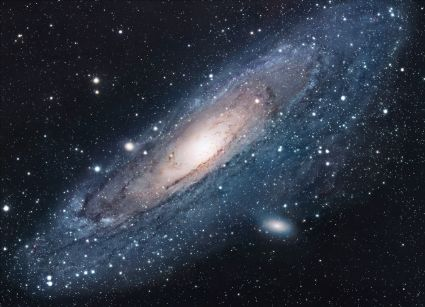
\includegraphics[scale=1.7]{universe}
\caption{The Universe}
\label{fig:universe}
\end{figure}

Here is an equation that has nothing to do with anything else here,
\begin{equation}
    \label{eq:1}
    \dfrac{\partial T}{\partial t} = \boldsymbol{\nabla} \cdot \kappa \boldsymbol{\nabla} T \ .
\end{equation}

And here is what eq. \eqref{eq:1} means. From this you cannot derive the following equation:

\begin{equation} \label{eq:2}
    z(x) = z(x_b) + \Bigg(\frac{k_s}{{A_0}^{\theta}}\Bigg) \int_{x_b}^{x} \Bigg(\frac{A_0}{A(x)}\Bigg)^{\theta} dx,
\end{equation}  

And here is what eq. \eqref{eq:2} doesn't mean. My first paper was \citet{Hurst2012}.

\section{Conclusion}
``I always thought something was fundamentally wrong with the universe'' \citep{adams1995hitchhiker}

\bibliographystyle{apalike}
\bibliography{references}
\end{document}
